\documentclass{article}

\textwidth=6.5in
\textheight=8.5in
\voffset=-54pt
\oddsidemargin=0in
\evensidemargin=0in
\setlength{\parskip}{8pt}
\setlength{\parindent}{0pt}

\usepackage{workbook}

\usepackage{handout}

\usepackage{exam}

\newcommand{\answerbox}[3][]{
    \fbox{\begin{minipage}[t][#2][c]{#3}
        #1
    \end{minipage}}
    }

\begin{document}

{\large \mbox{} \hfill \bf Name:\underline{\hspace{3in}}}\\[2pt]
{\mbox{} \hfill \it (Please write your name neatly in print.)}\\[12pt]
{\large \mbox{} \hfill \bf HUID:\underline{\hspace{3in}}}
 
\medskip
 
\noindent
{\large\bf
Exam 2 Practice 3\\
Math Mb Spring 2025}
\noindent


{\Large
\begin{center}\textbf{Directions---Please read carefully!} \end{center}}

This is a practice test. The same directions will appear on the actual exam, so read them carefully.

\hrulefill 


This exam is subject to the Harvard College Honor Code. No calculators or any other aids are permitted.  Please write as neatly as possible, as answers that can't be read can't be graded and thus can't receive credit. To receive full credit, you must show relevant working
and include units when appropriate. 

You have 120 minutes to complete this exam. 

You may ask for scratch paper if you need additional space to write, but it will not be scanned or graded. Make sure to include all relevant working in this exam booklet in the space provided for each question.

\begin{center}\textbf{Good luck!}\end{center}


\vfill

\centering{
\emph{As a member of Harvard College, I pledge that I will not give or receive assistance on this exam.}}
\vspace{0.3in}

{\large \mbox{} \hfill \bf Signature:\underline{\hspace{3in}}}
\thispagestyle{empty}

\newpage

\begin{enumerate}
\item

  %\solonly{\related{{{\#1}} on {the worksheet ``Net Change''};
     % {{\#1}} on {Workshop 10}; {Problem Set 19}, {{\#1}}}}

  \label{spring2009-xb-midterm2-1}



  A man is rowing a boat down the Charles River. He starts at the
  Longfellow bridge and wants to see the JFK bridge.  The two bridges
  are 3 miles apart.  The rate at which the man rows decreases
  exponentially with time and is given by the formula $r(t)=
  5\left(2^{-t} \right)$ miles per hour, where $t$ is the number of
  hours he has been rowing.

  \begin{enumerate}
  \item
    \begin{problem}[\vfill]
      Compute the right-hand approximation $R_2$ for the distance he
      travels in four hours.
    \end{problem}

    \begin{solution}
      Visually, we are trying to approximate the area under $r(t)$ from $t
      = 0$ to $t = 4$ using the area in these rectangles:
      \begin{center}
        \begin{tikzpicture}
          \begin{axis}[ytick={5}, width=2.5in]
            \addplot+[domain=-0.5:4.5]{5 / 2^x}; \addplot+[ybar interval,
            plusarea] coordinates { (0, 5/4) (2, 5/16) (4, 5/16) };
          \end{axis}
        \end{tikzpicture}
      \end{center}
      The area in the rectangles is
      \begin{align*}
        R_2 &= r(2) \cdot 2 + r(4) \cdot 2 \\
        &= 5(2^{-2})(2) + 5(2^{-4})(2) \\
        &= \frac{5}{2} + \frac{5}{8} \\
        &= \boxed{\frac{25}{8} \text{ miles}}
      \end{align*}
    \end{solution}

  \item
    \begin{problem}[\vfill]
      Compute the left-hand approximation $L_2$ for the distance he
      travels in four hours.
    \end{problem}

    \begin{solution}
      Visually, we are trying to approximate the area under $r(t)$ from $t
      = 0$ to $t = 4$ using the area in these rectangles:
      \begin{center}
        \begin{tikzpicture}
          \begin{axis}[ytick={5}, width=2.5in]
            \addplot+[domain=-0.5:4.5]{5 / 2^x}; \addplot+[ybar interval,
            plusarea] coordinates { (0, 5) (2, 5/4) (4, 5/4) };
          \end{axis}
        \end{tikzpicture}
      \end{center}
      The area in the rectangles is
      \begin{align*}
        L_2 &= r(0) \cdot 2 + r(2) \cdot 2 \\
        &= 5(2^{-0})(2) + 5(2^{-2})(2) \\
        &= 10 + \frac{5}{2} \\
        &= \boxed{\frac{25}{2} \text{ miles}}
      \end{align*}
    \end{solution}

  \item
    \begin{problem}[\vfill\newpage]
      Will the man pass the JFK bridge in four hours? Explain how you can
      be sure.
    \end{problem}

    \begin{solution}
      \fbox{Yes.}  We can see from our picture that $R_2$ is an
      underestimate for the actual distance the man travels in four hours.
      However, we calculated that $R_2 = \frac{25}{8} > 3$, so the man
      must row more than the 3 miles (the distance between the two
      bridges) in four hours.  

        \emph{Note:} Although FTOC 2 is not officially on the exam, you
        could also use FTOC 2 to calculate the exact distance he traveled
        in four hours, $\displaystyle \int_0^4 r(t)\,dt$.  (However, it's
        a little tricky to think of an antiderivative of $r(t)$.)
    \end{solution}

  \end{enumerate}

\item \label{spring2011-mb-final-8}
  
  % graph slightly modified by Janet

  %\solonly{\related{{Problem Set 23}}}

  {
    Below is the graph of a function $f(t)$ on the interval $[0, 12]$.

    \begin{center}
      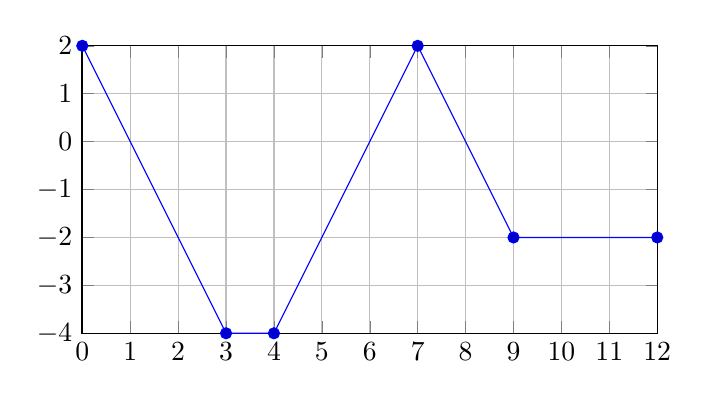
\begin{tikzpicture}
        \begin{axis}[xtick={0, 1, ..., 12}, ytick={-4, -3, ..., 2},
          grid=major, axis equal=true, clip=false, axis line style={shorten
            >=-8pt}, width=3.5in, height=2.06in, enlargelimits=false]
          \addplot+[sharp plot] coordinates { (0, 2) (3, -4) (4, -4) (7, 2)
            (9, -2) (12, -2)}; 
        \end{axis}
      \end{tikzpicture}
    \end{center}

    In this problem, you'll look at the function $A(x) =\displaystyle
    \int_1^x f(t) \,dt$.
    \begin{enumerate}

    \item What is $A(0)$? $\fitb{1in}{-1}$ \qquad \qquad What is
      $A(1)$? \fitb{1in}{0}

      \begin{solution}
        $A(0)$ is defined to be $\displaystyle \int_1^0 f(t)\,dt$, which
        is the same as $-\displaystyle \int_0^1 f(t)\,dt$.  From the graph of
        $f$, we can see that this is equal to $-1$.

        $A(1)$ is defined to be $\displaystyle \int_1^1 f(t)\,dt$, which
        is 0. 
      \end{solution}

      \pspace{\vfill}

    \item \label{spring2011-final-8-decreasing}
      \begin{problem}[\vfill]
        On which intervals in $[0, 12]$ is the graph of $A(x)$
        decreasing?
      \end{problem}

      \begin{solution}
        Our usual strategy for figuring out where a function is decreasing
        is to make a sign chart for its derivative.  In this case, the
        derivative of $A$ is just $f$, by FTOC 1.  So, let's make a
        sign chart for $f$:
        \begin{center}
          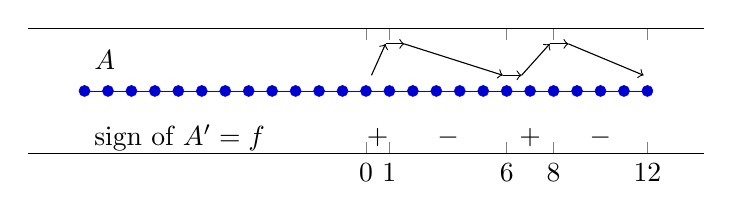
\begin{tikzpicture}
            \begin{axis}[axis y line=none, x axis line style={-}, xtick={0., 1., 6., 8., 12.}, xticklabels={$0$, $1$, $6$, $8$, $12$}, ymin=-2, ymax=2, height=1.25in, width=4in]
              \addplot+[domain=-12:12., very thin]{0};
              \draw (axis cs: -12, -1.5) node[right] {sign of $A' = f$};
              \draw (axis cs: -12, 1) node[right] {$A$};
              \draw (axis cs: 0.5, -1.5) node{$+$};
              \draw[->, xshift=2pt] (axis cs: 0, 0.5) -- (axis cs: 0.6, 1.5);
              \draw (axis cs: 3.5, -1.5) node{$-$};
              \draw[->, xshift=2pt] (axis cs: 1.4, 1.5) -- (axis cs: 5.6, 0.5);
              \draw (axis cs: 7., -1.5) node{$+$};
              \draw[->, xshift=2pt] (axis cs: 6.4, 0.5) -- (axis cs: 7.6, 1.5);
              \draw (axis cs: 10., -1.5) node{$-$};
              \draw[->, xshift=2pt] (axis cs: 8.4, 1.5) -- (axis cs: 11.6, 0.5);
              \draw[->, xshift=2pt] (axis cs: 0.6, 1.5) -- (axis cs: 1.4, 1.5);
              \draw[->, xshift=2pt] (axis cs: 5.6, 0.5) -- (axis cs: 6.4, 0.5);
              \draw[->, xshift=2pt] (axis cs: 7.6, 1.5) -- (axis cs: 8.4, 1.5);
            \end{axis}
          \end{tikzpicture}
        \end{center}
        From this, we can see that $A(x)$ is decreasing on \fbox{$(1,
          6)$ and $(8, 12)$}.
      \end{solution}

    \item
      \begin{problem}[\vfill]
        On which intervals in $[0, 12]$ is the graph of $A(x)$ concave
        down?
      \end{problem}

      \begin{solution}
        By {Problem Set 23}, {{{{\#6}}(b)}}, $A$ is
        concave down when $f$ is decreasing, which happens on \fbox{$(0,
          3)$ and $(7, 9)$}.
      \end{solution}

    \item For which $x$ in $[0, 12]$ does $A(x)$ have a local maximum?
      \fitb{1in}{1, 8}

      \pspace{\vfill}

      \begin{solution}
        From our sign chart in \ref{spring2011-final-8-decreasing}, we see
        that $A$ has local maxima at $x = 1, 8$.
      \end{solution}

    \item For which $x$ in $[0, 12]$, if any, does $A(x)$ have an
      absolute maximum? \fitb{1in}{1}

      \pspace{\vfill\newpage}

      \begin{solution}
        From our sign chart, we can see that $A$ must have an absolute
        maximum at either $x = 1$ or $x = 8$.  To decide between these, we
        need to figure out whether $A(1)$ or $A(8)$ is bigger:
        \begin{align*}
          A(1) &= \int_1^1 f(t)\,dt = 0 \\
          A(8) &= \int_1^8 f(t)\,dt, \text{ which is negative (by
            looking at the graph of $f$)}
        \end{align*}
        So, $A(1)$ is greater than $A(8)$, and the absolute
        maximum of $A$ occurs at $x = 1$.
      \end{solution}

    \item
      \begin{problem}[\vfill]
        Is the graph of $A(x)$ ever positive on $[0, 12]$? Why or why
        not? Please explain briefly.
      \end{problem}

      \begin{solution}
        No, we already said that the absolute maximum was at $x = 1$, and
        $A(1) = 0$.  So, the highest point on the graph is $(1, 0)$.
      \end{solution}    

    \item 

      \begin{problem}
        Sketch a rough graph of $A(x)$ on $[0, 12]$ on the axes
        provided below.  Clearly indicate all intercepts, as well as the
        $x$-coordinates of all local extrema.  Your graph should
        accurately portray the concavity of $A$ and everything else you
        have found in this problem.
      \end{problem}

      \probonly{\axes[xmin=0, xmax=12.5, xtick={1, 2, ..., 12}, width=4in]}

      \pspace{\vfill}

      \begin{solution}
        \begin{center}
          \begin{tikzpicture}
            \begin{axis}[cycle list=black, ytick={-1}, height=2.25in,
              width=3.5in, xtick={1, 2, ..., 12}]
              \addplot+[domain=9.:12.]{7. - 2.*x};
              \addplot+[domain=3.:4.]{8. - 4.*x};
              \addplot+[domain=0.:3.]{-1.*(-1. + x)^2};
              \addplot+[domain=7.:9.]{-74. + 16.*x - 1.*x^2};
              \addplot+[domain=4.:7.]{24. - 12.*x + x^2};
            \end{axis}
          \end{tikzpicture}
        \end{center}
   

        Here are the key features of the graph: 
        \begin{itemize}
        \item It has $y$-intercept $-1$ and $x$-intercept $1$. 
        \item It should be increasing on $(0, 1)$, decreasing on $(1, 6)$,
          increasing on $(6, 8)$, and decreasing on $(8, 12)$.
        \item It should be concave down on $(0, 3)$, linear on $(3, 4)$ with
          slope $-4$, concave up on $(4, 7)$, concave down on $(7, 9)$, and
          linear on $(9, 12)$ with a slope of $-2$.
        \item The absolute maximum of the graph is $(1, 0)$, so the rest of
          the graph is below the $x$-axis.  
        \end{itemize}
        Consistency is important in such problems; be sure that your graph
        agrees with your work in the previous parts. 
     \end{solution}

    \item 

      Suppose that the function $f(t)$ above represents the rate of change
      of temperature, in degrees per hour, $t$ hours after noon one day.
      At noon, it is $36^\circ$.
      \begin{enumerate}

      \item
        \begin{problem}[\vfill]
          What quantity is represented by $A(x)$?  Your answer should be
          in terms of temperature and time.
        \end{problem}

        \begin{solution}
          $A(x) = \displaystyle \int_1^x f(t)\,dt$ is the \fbox{net
            change in temperature between 1 pm and time $x$}.
        \end{solution}

      \item
        \begin{problem}[\vfill]
          What quantity is represented by $A(4)$?
        \end{problem}

        \begin{solution}
          $A(4)$ is the \fbox{net change in temperature between 1 pm
            and 4 pm}.
        \end{solution}

      \item
        \begin{problem}[\vfill\newpage]
          What is the temperature at 5 pm?  (Your answer should be a number,
          and it should not include any integral signs.)
        \end{problem}

        \begin{solution}
          We know that the temperature at noon is $36^\circ$, so if we can
          find the net change in temperature from noon to 5 pm, then we will
          know the temperature at 5 pm.
          \begin{align*}
            \text{temperature at 5 pm} &= 36 + \text{net change in temp from
              noon to 5 pm} \\
            &= 36 + \int_0^5 f(t)\,dt \\
            \intertext{From the graph of $f$, we find that $\displaystyle
              \int_0^5 f(t)\,dt = -10$:}
            &= 36 - 10 \\
            &= \boxed{26^\circ}
          \end{align*}
        \end{solution}

      \end{enumerate}
    \end{enumerate}
  }
%%%%%%%%%%%%%%%%%%%%%%%%%%%%%%%%%



\item \label{spring2014-m2practice1-limits}



  Evaluate the following limits. If a limit does not exist because it is
  $\infty$ or $-\infty$, indicate this as well.

  \begin{enumerate}
  \item \label{fall2012-1a-midterm2-5a}

    \begin{problem}[\vfill]
      $\displaystyle \lim_{x \rightarrow 1} \frac{x^4 - 4x + 3}{(x -
        1)^2}$
    \end{problem}

    \begin{solution}
      This is a $\frac{0}{0}$ limit, so we can use L'H\^opital's Rule:
      \begin{align*}
        \lim_{x \to 1} \frac{x^4 - 4x +3}{(x-1^2)} 
        & \lheq \lim_{x \to 1} \frac{4 x^3 - 4}{2x-2} \\
        \intertext{This is another $\frac{0}{0}$ limit, so we can use
          L'H\^opital's Rule again:}
        & \lheq \lim_{x \to 1} \frac{12 x^2}{2} \\
        & \nolheq \boxed{6}
      \end{align*}
    \end{solution}

  \item
    \begin{problem}[\vfill]
      $\displaystyle \lim_{x \rightarrow 0} \frac{\arccos x}{\cos x - 1}$
    \end{problem}

    \begin{solution}
      As $x \to 0$, $\arccos x \to \arccos (0) = \frac{\pi}{2}$ and
      $\cos x - 1 \to 0$.  In this situation (where the numerator tends
      to a non-zero limit and the denominator tends to 0), we must think
      about the sign of the denominator.  Here, $\cos x - 1$ is negative
      when $x$ is close to 0, so the limit is $\boxed{-\infty}$. 
    \end{solution}

  \item

    \begin{problem}[\vfill]
      $\displaystyle \lim_{x \to 0^+} (1 - \arcsin x)^{1/x}$
    \end{problem}

    \begin{solution}
      As $x \to 0^+$, $1 - \arcsin x \to 1 - \arcsin(0) = 1$ and
      $\frac{1}{x} \to \infty$, so this is a $1^\infty$ limit.
      Therefore, we should rewrite it so that we can apply L'H\^opital's
      Rule:
      \begin{align}
        (1 - \arcsin x)^{1/x} &= e^{\raisebox{3pt}{$\ln \left[ (1 -
              \arcsin x)^{1/x} \right]$}} \nonumber \\
        &= e^{\raisebox{4pt}{$\frac{1}{x} \ln (1 - \arcsin x)$}} \label{eq:spring2014-m2practice1-limits-1-to-the-inf-rewrite}
      \end{align}
      Now, let's focus on what happens to the exponent in the last
      expression as $x \to 0^+$:
      \begin{align*}
        \lim_{x \to 0^+} \frac{1}{x} \ln (1 - \arcsin x) & \nolheq
        \lim_{x \to 0^+} \frac{\ln(1 - \arcsin x)}{x} \\
        \intertext{As $x \to 0^+$, $\ln (1 - \arcsin x) \to \ln(1) = 0$
          and $x \to 0$, so this is a $\frac{0}{0}$ limit, and we can
          use L'H\^opital's Rule:} & %
        \lheq \lim_{x \to 0^+} \frac{\displaystyle \frac{1}{1 - \arcsin
            x} \left( -\frac{1}{\sqrt{1 - x^2}} \right)}{1} \\
        & \nolheq \lim_{x \to 0^+} - \frac{1}{(1 - \arcsin
          x) \sqrt{1 - x^2}} \\
        \intertext{As $x \to 0^+$, $\sqrt{1 - x^2} \to 1$ and $1 -
          \arcsin x \to 1$, so this limit is} %
        & \nolheq -1
      \end{align*}
      Remember that this was only the limit of the exponent in
      \eqref{eq:spring2014-m2practice1-limits-1-to-the-inf-rewrite}, so
      the limit we want is $e^{-1} = \boxed{\frac{1}{e}}$.
    \end{solution}

  \item
    \begin{problem}[\vfill\newpage]
      $\displaystyle \lim_{x \to 2} \left( \sin \pi x
      \right)^{1/(x-2)^2}$ 
    \end{problem}

    \begin{solution}
      As $x \to 2$, $\sin \pi x \to 0$ and $\frac{1}{(x - 2)^2} \to
      \infty$, so this limit is $\boxed{0}$.  ($0^\infty$ is not
      indeterminate: if you raise a number close to 0 to a huge problem,
      your answer is even closer to 0.)
    \end{solution}

  \end{enumerate}

% \item \label{spring2009-midterm2-6} \finishexam 



\item   Ma's 24-hour bakery makes muffins at a rate of $m(t)$ muffins per hour
  throughout the day ($t$ measures the time in hours since midnight).
  Muffins are stored on the shelf until they are purchased. Customers
  arrive at the bakery at a rate of $c(t)$ customers per hour.  The
  customers each want one muffin, are served as soon as they arrive, and
  leave as soon as they are served.

  Old muffins are thrown out at midnight, so the bakery has no muffins
  at time $t = 0$.

  The following is a graph of $m(t)$ and $c(t)$ over the interval
  $[0,24]$. (Note that $c(t) = 0$ for $0 \leq t \leq 5$.)

  \begin{center}
    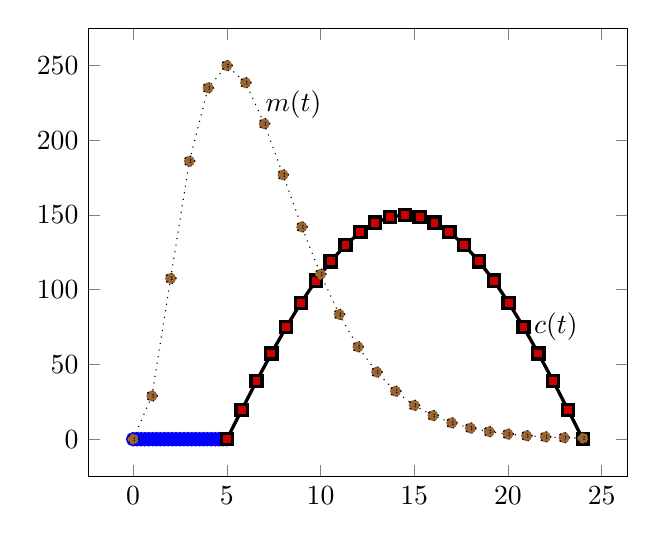
\begin{tikzpicture}
      \begin{axis}
        \addplot+[domain=0:5, very thick] {0}; \addplot+[black,
        domain=5:24, very thick] {150*sin(deg(2*pi*(x-5)/38))}
        node[pos=0.75, right] {$c(t)$}; \addplot+[black, dotted,
        domain=0:24] {
          3.4297996003123545*2.718281828459045^(2.6648801117587464 -
          0.5329760223517493*x)*x^2.6648801117587464} node[pos=0.55,
        right] {$m(t)$};
      \end{axis}
    \end{tikzpicture}
  \end{center}

  \begin{enumerate}
  \item Which of the following expressions describe the number of
    muffins the bakery has prepared when the first customer arrives?
    Circle \textbf{all}.

    \begin{multicols}{2}
      \begin{enumerate}[label=\protect{\maybecircle{\Alph*.}},
        itemsep=0.2cm]
      \plainitem $m(5) - m(0)$ $\vphantom{\displaystyle \int_0^1}$
      \circleitem $\displaystyle \int_0^5 m(t) \,dt$
      \plainitem $m(5) - c(5)$ $\vphantom{\displaystyle \int_0^1}$
      \circleitem $\displaystyle \int_0^{24} m(t)\,dt - \int_5^{24}
        m(t)\,dt$

      \plainitem $\displaystyle \int_0^5 c(t)\,dt$
      \plainitem $\displaystyle \int_0^{10} m(t) \,dt$
      \end{enumerate}
    \end{multicols}

    \begin{solution}
      The first customer arrives at time $t = 5$, so we are looking for
      the number of muffins made between time $t = 0$ and $t = 5$, which
      is $\displaystyle \int_0^5 m(t)\,dt$.  Expressions B,
        and D are all ways of writing this.
    \end{solution}

  \item
    \begin{problem}[\vfill]
      Write an expression for the total number of customers that visit
      Ma's store over the course of the day.
    \end{problem}

    \begin{solution}
      Since $c(t)$ gives the rate at which customers arrive during the
      day, the total number of customers is $\boxed{\int\limits_0^{24}
        c(t) \,dt}$. (Since $c(t) = 0$ for $0 \leq t \leq 5$, the
      expression $\boxed{\int\limits_5^{24} c(t) \,dt}$ is also correct.)
    \end{solution}

  \item
    \begin{problem}[\vfill\newpage]
      At what time is the number of muffins on the shelf at its maximum
      for the day? Justify your answer.
    \end{problem}

    \begin{solution}
      The graphs of $m(t)$ and $c(t)$ cross at $t = 10$. For $t < 10$,
      $m(t) > c(t)$, which means that muffins are being made faster than
      customers are arriving; as a result, the number of muffins on the
      shelf continues to grow.

      For $t > 10$, $c(t) > m(t)$, which means that customers are arriving
      faster than muffins are being made; as a result, the number of
      muffins on the shelf decreases.

      So, the maximum number of muffins on the shelf occurs at $t = 10$,
      or \fbox{10 am}.
    \end{solution}

  \item

    Interpret each of the following statements in the context of the
    problem. In each part, your answer should be a complete English
    sentence with no mathematical symbols. For example, the statement
    ``$c(15) = 150$'' could be interpreted as, ``At 3 pm, customers are
    arriving at the bakery at a rate of 150 customers per hour.''
    \begin{enumerate}
    \item
      \begin{problem}[\vfill]
        ``$\displaystyle \int_4^{10} m(t)\,dt = 1210$''
      \end{problem}

      \begin{solution}
        ``Between 4 am and 10 am, $1210$ muffins are made.''
      \end{solution}

    \item
      \begin{problem}[\vfill]
        ``$\displaystyle \int_0^{24} \left[ m(t)-c(t) \right]\,dt = 5$''
      \end{problem}

      \begin{solution}
        ``At the end of the day, there are 5 more muffins on the shelf
        than there were at the beginning of the day.''  (Since we are told
        that there are no muffins at time $t = 0$, another correct
        interpretation is, ``At the end of the day, there are $5$ muffins
        left on the shelf.'')
      \end{solution}

    \item
      \begin{problem}[\vfill\newpage]
        ``$m(t)$ has a maximum at $t=5.5$''
      \end{problem}

      \begin{solution}
        ``The bakery is producing muffins most quickly at 5:30 am''
      \end{solution}

    \end{enumerate}

  \end{enumerate}



%\instructions{instructions.tex}{../sections.tex}

% \listofproblems


\item \label{spring2014-midterm2-1-modified}
 
    The Vlasic pickle factory has two five-hour shifts over a ten-hour
    workday, during which two groups of employees work pickling cucumbers (a
    pickle is a cucumber soaked in vinegar, a process known as
    pickling). The AM shift works in the morning for five hours, and then
    the PM shift works for the next five hours.

    The function $P(t)$, graphed below, gives the factory productivity
    rate in thousands of pickles per hour, with $t$ given in hours after
    the AM shift starts.
    \begin{center}
      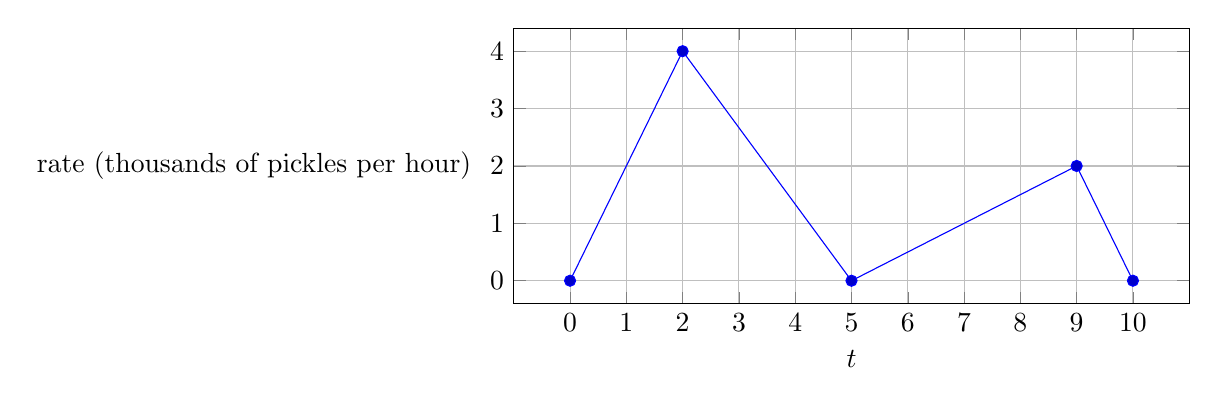
\begin{tikzpicture}
        \begin{axis}[grid=major, xtick={0, 1, ..., 10}, ytick={0, 1, ..., 4}, y label style={rotate=-90},
          xlabel=$t$, ylabel={rate (thousands of pickles per hour)},
          width=4in, height=2in] 
          \addplot+[sharp plot] coordinates { (0, 0) (2, 4) (5, 0) (9, 2)
            (10, 0) };
        \end{axis}
      \end{tikzpicture}
    \end{center}

    \begin{enumerate}

    \item
      \begin{problem}[\vfill]
        What is the maximum pickling rate over the course of the day? (Be
        sure to include units in your answer.)  When does this maximum rate
        occur?
      \end{problem}

      \begin{solution}
        The maximum pickling rate occurs when the rate graph is highest,
        which is at $\boxed{t = 2}$; this maximum rate is \fbox{4000 pickles
          per hour}.
      \end{solution}

    \item
      \begin{problem}[\vfill]
        At what time (value of $t$) have the workers produced a total of
        1000 pickles? How can you tell?
      \end{problem}

      \begin{solution}
        The number of pickles the workers have produced by time $T$ is
        $\displaystyle \int_0^T P(t)\,dt$, and we want this to equal
        $1000$.  This happens at time $\boxed{1}$ because the area under the
        curve from $t = 0$ to $t = 1$ is $1000$.  
      \end{solution}

    \item
      \label{spring2014-mb-midterm2-1-c}
      \begin{problem}[\stretch{0.7}]
        Write a definite integral that, when evaluated, gives the number of
        cucumbers pickled by the PM team.
      \end{problem}

      \begin{solution}
        The PM team works from $t = 5$ to $t = 10$; in this time, the number
        of cucumbers pickled is $\boxed{\int_5^{10} P(t)\,dt}$.
      \end{solution}

    \item
      \begin{problem}[\vfill\newpage]
        Evaluate the integral you wrote in \ref{spring2014-mb-midterm2-1-c}
        to find the number of cucumbers pickled by the PM team.
      \end{problem}

      \begin{solution}
        The area under $P(t)$ from $t = 5$ to $t = 10$ is $5$, representing
        \fbox{5000 cucumbers pickled}.
      \end{solution}

    \end{enumerate}

    \continueproblem{\emph{Continued from previous page:}
      \begin{center}
        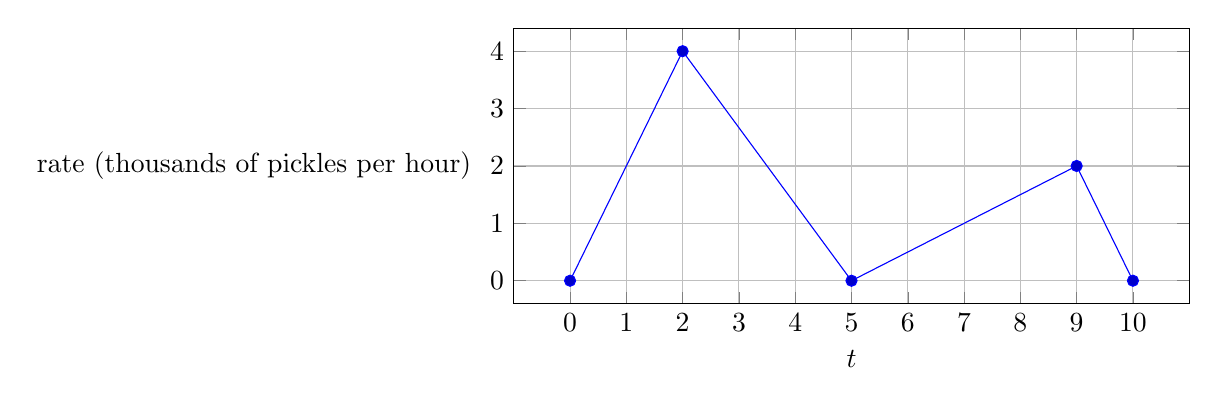
\begin{tikzpicture}
        \begin{axis}[grid=major, xtick={0, 1, ..., 10}, ytick={0, 1, ..., 4}, y label style={rotate=-90},
          xlabel=$t$, ylabel={rate (thousands of pickles per hour)},
          width=4in, height=2in] 
          \addplot+[sharp plot] coordinates { (0, 0) (2, 4) (5, 0) (9, 2)
            (10, 0) };
        \end{axis}
      \end{tikzpicture}
      \end{center}
    }

    \begin{enumerate}[resume]

    \item
      \begin{problem}[\vfill]
        If the PM shift, throughout the PM time period, were to pickle at
        twice the rate shown in the graph, how would the number of pickles
        they produce change?
      \end{problem}

      \begin{solution}
        This would double their production of pickles to 10,000. 
      \end{solution}

    \item
      \begin{problem}[\vfill]
        When the pickles are made, they are put in a vat.  A pipe then
        takes pickles from the vat to a larger storage tank. The pipe
        transports pickles at a rate of $2000$ pickles per hour. When do
        pickles start to pile up in the vat? How do you know?
      \end{problem}      

      \begin{solution}
        The pickles start to pile up when the rate of pickle production
        exceeds 2000 pickles per hour. This occurs when $\boxed{t=1}$.  
      \end{solution}

    \item
      \begin{problem}[\stretch{1.5}]
        When is the vat most full?  At that time, how many pickles are in
        the vat?
      \end{problem}

      \begin{solution}
        From $t = 1$ to $t = 3.5$, pickles are produced at a rate of at
        least $2000$ pickles per hour, so pickles continue to pile up in
        the vat.  After $t = 3.5$, the rate of production is always $\leq
        2000$ pickles per hour, so pickles are removed from the vat more
        quickly than they are produced, and the vat gets less full.
        Therefore, the vat is most full at $\boxed{t = 3.5}$.  The number
        of pickles in the vat at $t = 3.5$ is (number of pickles produced
        between $t = 1$ and $t = 3.5$) $-$ (number of pickles removed
        between $t = 1$ and $t = 3.5$), or $\displaystyle \int_{1}^{3.5}
        P(t)\,dt - \int_1^{3.5} 2\, dt$ since pickles are removed at a
        rate of 2 thousand pickles per hour.  We can picture this as
        the area under $P(t)$ from $t = 1$ to $t = 3.5$ (shaded in blue
        below) minus the area under $2$ from $t = 1$ to $t = 3.5$ (shaded
        in red below):
        \begin{center}
          \begin{tikzpicture}
            \begin{axis}[grid=major, xtick={0, 1, ..., 10}, ytick={0, 1, ..., 4},
              xlabel=$t$, ylabel={rate (thousands of pickles per hour)}, y label style={rotate=-90},
              width=4in, height=2in] 
              \addplot+[sharp plot, pattern= north west lines, pattern
              color=blue] coordinates { (1, 2) (2, 4) (3.5, 2) }
              \closedcycle; %
              \addplot+[domain=1:3.5, red] {2};
              \addplot+[domain=1:3.5, pattern= north west lines, pattern color=red, draw=none] {2} \closedcycle; %
              \addplot+[sharp plot, black] coordinates { (0, 0) (2, 4) (5,
                0) (9, 2) (10, 0) };
            \end{axis}
          \end{tikzpicture}
        \end{center}
        The difference is the area shaded just in blue, which is a
        triangle of width 3.5 and height 2; therefore, its area is
        $\frac{1}{2} (3.5) (2) = 3.5$, representing \fbox{3500 pickles}. 
      \end{solution}

    \item
      \begin{problem}[\nstretch{1.5}]
        Once the pickles start to pile up in the vat, does the vat ever
        become empty again (on this day)?  How do you know?
      \end{problem}

      \begin{solution}
        The vat \fbox{does empty out again}.  For example, the number of
        pickles produced between $t = 1$ and $t = 9$ (which can be
        visualized as the area under $P(t)$ from $t = 1$ to $t = 9$) is
        less than the number of pickles that the pipe could take away
        (which can be visualized as the area under $y = 2$ from $t = 1$ to
        $t = 9$).  That means that the pipe has been able to empty the vat
        out sometime before $t = 9$.
      \end{solution}

    \end{enumerate}

\item \label{spring2012-mb-midterm2-4}


  John is running a marathon.  His running speed after $t$ hours of
  running is given by $v(t) = 8-\frac{1}{2}t^2$ miles per hour.

  \begin{enumerate}

  \item
    \begin{problem}[\vfill]
      Use a right-hand approximation with 4 terms, $R_4$, to approximate
      the distance John runs in the first 2 hours of the race.

      You do \textbf{not} need to simplify your answer; it's fine to leave
      it as a sum of numbers, as well as to leave expressions like $v(3)$
      in your answer.
    \end{problem}

    \begin{solution}
      Graphically, we can picture the distance John runs as the area under
      the velocity curve between $t=0$ and $t=2$.  Since we are dividing
      the interval $[0,2]$ into 4 slices, each slice will have width
      $\frac{1}{2}$.  Here's a picture of $R_4$:
      \begin{center}
        \begin{tikzpicture}[declare function={f(\x)=8-\x^2/2;}]
          \begin{axis}[ymin=0, ytick={8}, width=3in]
            \addplot+[ybar interval, plusarea] coordinates { (0, {f(1/2)})
              (1/2, {f(1)}) (1, {f(3/2)}) (3/2, {f(2)}) (2, {f(2)}) }; %
            \addplot+[domain=0:2.4, black] {f(x)} node[pos=0.7,
            anchor=south west]{$y = v(t)$};
          \end{axis}
        \end{tikzpicture}
      \end{center}
      The area of the rectangles is $\boxed{v(0.5) 0.5 + v(1) 0.5 + v(1.5)
        0.5 + v(2) 0.5}$. 
    \end{solution}

  \item
    \begin{problem}[\vfill\newpage]
      Is $R_4$ an underestimate or overestimate for the actual distance
      John runs in the first 2 hours of the race, or is it impossible to
      determine that from the given information?  Justify your answer. 
    \end{problem}

    \begin{solution}
      From our picture, we can see that $R_4$ is an \fbox{underestimate}
      for the actual distance. 
    \end{solution}

  \end{enumerate}

 %  \item Let $y=\arcsin(x)$. Determine the derivative of $y$ with respect to $x$ by starting with $x = \sin(y)$ and using implicit differentiation.

 % \begin{solution}
 %    To determine $\frac{d}{dx} (\arcsin x)$, we start with the
 %    equation
 %    \begin{align*}
 %      y &= \arcsin x \\
 %      \intertext{We'd like to find $\frac{dy}{dx}$, and we'll first
 %        rewrite this in terms of $\sin$ since we know how to differentiate
 %        $\sin$:}
 %      \sin y &= x \\
 %      \shortintertext{Differentiate both sides with respect to $x$:}
 %      \frac{d}{dx} (\sin y) &= \frac{d}{dx} (x) \\
 %      \cos y \frac{dy}{dx} &= 1 \\
 %      \frac{dy}{dx} &= \frac{1}{\cos y}
 %    \end{align*}
 %    We need to figure out how to express
 %    this in terms of $x$.  The equation $y = \arcsin x$ says that $y$ is
 %    the angle in $\left[ - \frac{\pi}{2}, \frac{\pi}{2} \right]$ whose
 %    sine is $x$, and we can picture this statement graphically:
 %    \begin{center}
 %      \begin{tikzpicture}
 %        \begin{axis}[axis equal=true, xmin=-4.5, xmax=4.5, ymin=-4.5,
 %          ymax=4.5, xtick=\empty, ytick=\empty, width=2.25in,
 %          height=2.25in, clip=false] %
 %          \draw[blue, thick] (axis cs: 0, 0) -- (axis cs: 4, 0) --
 %          node[right]{$x$} (axis cs: 4, 3) -- node[anchor=south east]
 %          {$1$} (axis cs: 0, 0); %
 %          \pgfmathsetmacro{\angle}{atan(3/4)} %
 %          \addplot+[domain=0:\angle, red, thin, ->, >=to] ({0.6 *
 %            cos(x)}, {0.6 * sin(x)}) node[pos=0.5, right] {$y$};
 %        \end{axis}
 %      \end{tikzpicture}        
 %    \end{center}
 %    By the Pythagorean Theorem, this triangle has width $\sqrt{1 - x^2}$,
 %    so $\cos y = \frac{\sqrt{1 - x^2}}{1} = \sqrt{1 - x^2}$.  Therefore,
 %    $\displaystyle \frac{dy}{dx} = \frac{1}{\cos y} =
 %    \boxed{\frac{1}{\sqrt{1-x^2}}}$.
 %  \end{solution}
  
\item
  \label{spring2007-midterm2-6} 


  Answer the true/false questions below by filling in the appropriate
  bubble.  If the statement is false, explain why or give an example
  demonstrating that it is false (your example may be a picture).  If the
  statement is true, you do not need to provide any explanation.

    \tfheading{}
    
  \begin{tf}{f} % TF 1
    Estimating a definite integral with a right-hand sum always gives an
    overestimate.

    \begin{solution}
      If we use a right-hand sum to approximate the definite integral
      represented by the area below, we'll get an underestimate:
      \begin{center}
        
\includegraphics[width=1.5in]{images/area-sums-reflect-back-3}
      \end{center}
    \end{solution}
  \end{tf}

  \pspace{\vfill}

  \begin{tf}{f} % TF 2
    Estimating a definite integral with a right-hand sum always gives an
    underestimate.

    \begin{solution}
      If we use a right-hand sum to approximate the definite integral
      represented by the area below, we'll get an overestimate:
      \begin{center}
        
\includegraphics[width=1.5in]{images/area-sums-reflect-back-1}
      \end{center}
    \end{solution}
  \end{tf}

  \pspace{\vfill}

  \begin{tf}{t} % TF 3
    Suppose $f$ is a continuous function, and $L_n$ and $R_n$ are
    left-hand and right-hand sums with $n$ rectangles for $\displaystyle
    \int_a^b f(x)\,dx$.  Then, $\displaystyle \lim_{n \to \infty} L_n =
    \lim_{n \to \infty} R_n$. 

    \begin{solution}
      Both $\displaystyle \lim_{n \to \infty} L_n$ and $\displaystyle
      \lim_{n \to \infty} R_n$ are equal to $\displaystyle \int_a^b
      f(x)\,dx$.  (That's the definition of the definite integral.)
    \end{solution}
  \end{tf}

  \pspace{\vfill}

  \begin{tf}{f} % TF 4 % added by Janet
    If $f$ is a continuous function which is increasing on $(-\infty,
    \infty)$, then $A(x)=\int_0^x f(t)\,dt$ is also increasing on $(-\infty, \infty)$.

    \begin{solution}
      By {Problem Set 23}, {{{{\#6}}(b)}}, $A(x)$ is increasing where
      $f$ is positive.  So, if $f(x) = x$ (which is increasing on
      $(-\infty, \infty)$ but only positive for $x > 0$), then $A(x)$
      will only be increasing for $x > 0$. 
    \end{solution}
  \end{tf}
  \pspace{\vfill}
  
\end{enumerate}






\end{document}